%  \menulabel{ \bmenut{}{}\blink\bmenut{}{}}
\chapter{Schnellstart}\label{cha:quickstart}

Dies Kapitel soll einen schnellen Einstieg in \xc geben und stellt einige typische Vorgehensweisen vor.
Es wird davon ausgegangen, daß einige pilotenbezogene Einstellungen bereits vorgenommen wurden.
Es werden einfach Aufgaben programmiert und ein paar Grundeinstellungen vorgenommen.

Diese Anleitungen werden Schritt für Schritt beschrieben und beim Erstellen diverser, verschieden komplexer
Aufgaben helfen. Definitiv  werden nicht alle Funktionen und Möglichkeiten von \xc hier beschrieben.

\section{Reinsetzen \& Fliegen}
Ja, das geht auch. Das dumme daran ist, daß \xc nicht weiß, was Du vorhast bzw.\ wo Du hin willst.
Als Landkarte kann man \xc aber dennoch gut benutzen, um z.B. Lufträumen auszuweichen.

Für den Fall, daß keine Aufgabe deklariert wurde und kein Heimatflugplatz deklariert wurde, nimmt \xc den aktuellen Startplatz als Heimat an ("lift off"),
sodaß Du auch ohne irgendetwas zu machen problemlos wieder nach Hause kommen wirst.
Es erscheint dann eben nicht der Name des Heimatflugplatzes, sondern einfach ein ''takeoff'' auf der Karte.

\section{MachMich Heimat}\index{Heimatflugplatz}\index{MachMichHeimat}
Wenn keinerlei Wendepunkt, Start, Ziel oder Aufgabe einprogrammiert ist und/oder werden soll, kann man auf
folgende Art und Weise den Heimatflugplatz erstellen.
Beim Start nimmt  \xc dann grundsätzlich diesen Platz -den Heimatflugplatz- als Ziel und alle
navigatorischen Berechnungen beziehen sich auf diesen Punkt - bis ein neuer Wendepunkt eingestellt wurde.

\menulabel{ \bmenut{Nav}{1/2}\blink\bmenut{Wegpunkt}{Liste}}
Das geht am schnellsten mittels des  des Nav-Menüs.  Den den entsprechenden Wegpunkt mit \button{auswählen} anklicken,
zweimal  $\triangleright\triangleright$ und anschließend  \button{Setze als Heimatflugplatz}
Damit ist der Heimatplatz bis auf weiteres in der Konfiguratuion einprogrammiert und wird, wenn keine Aufgabe deklariert ist, als Ziel
Standardziel benutzt.

%%%%%%%%%%%%%%%%%%%%%
\section{Platzrunden und lokaler Flug}\label{sec:local-flight}

In diesem Beispiel möchte der Pilot einen lokalen Rundflug unternehmen oder einfach einen spontanen Flug durch die Gegend
unternehmen, wobei keine Wendepunkte in einer Aufgabe explizit angeflogen werden müssen und keine
Start- und Zielregeln eingehalten werden müssen.

Dies stellt ebenfalls eine Möglichkeit dar, den Heimatflugplatz einzuprogrammieren.

\subsection*{Vor dem Start}
\begin{enumerate}
\item  Schalte das Gerät an (..!..)
\item  Öffne mit den \menulabel{\bmenut{Konfig.}{1/3}\blink\bmenut{Flug}{Einstellung}} das entsprechende Menu,
und stelle Wasserballast, Mückenbeladung und die maximal zu erwartende  Tagestemperatur ein. Schließe diesen Dialog.
\item  Öffnen die Aufgabenverwaltung  \button{Verwalten} und erstelle eine \menulabel{ \bmenut{Nav}{1/2}\blink\bmenus{Aufgabe}}neue  Aufgabe mit \button{Verwalten}, \button{Neue Aufgabe}
\item  Wähle z.B.\ "Racing" als Aufgabentyp (Im Fenster ganz unten) und bestätige dies mit "Auswählen".
\item  Nun holst Du Dir entsprechende Wendepunkte im Wegpunktedialog: \button{Wendepunkt}
Hier wählst Du einen Wendepunkt aus. \button{Wendepunkt hinzufügen} Beachte die vier wirklich \textsl{sehr} hilfreichen Filter
hierbei, oder tippe einfach einen gewünschten Namen ein.
\item Wähle einen zweiten Wegpunkt aus und kennzeichne diesen als "Ziel"  (z.B. Deinen Heimatfluplatz)
\button{Als Endpunkt}
\item Nun enthält diese Aufgabe einen Wendepunkt, Dein Ziel.
\item Speichern der Aufgabe nicht vergessen!
\item anschließend auf \button{Fliegen} drücken und ab gehtŽs.
\end{enumerate}

\subsection*{Während des Fluges}
\begin{enumerate}
\item  Bei Bedarf, nachjustieren des MC-Wertes, um dem Rechner den entsprechenden Wert zu übermitteln und gemäß der MC-Theorie zu fliegen.
\item  Dasselbe mit Mückenbeladung  und Wasserballast.
\item  Das Flugzeug kann zu jeder Zeit den Heimatflugplatz erreichen, sofern der Endanflugspfeil auf der linken Seite des Displays grün erscheint und nach oben zeigt.
\item  Optional kann der MC-Wert auf AUTO gestellt werden, \button{MC Auto}, um den Heimflug zu beginnen.
\menulabel{\bmenut{Konfig.}{1/3}\blink\bmenut{MC}{Auto}}
Wenn der MC-MC-Modus auf "Endanflug" oder "Beides" gesetzt wurde, wird der
Rechner die optimale Geschwindigkeit zum Erreichen des Zieles angeben. (Sollfahrt für besten Schnitt)
\end{enumerate}

%%%%%%%%%%%%%%%%%%%
\subsection*{Nach der Landung}

\begin{enumerate}
\item  Der Analyse-Dialog  mit den entsprechenden Untermenüs gibt Info über Thermikstärke, das Barogramm,
  \menulabel{ \bmenut{Info}{1/3}\blink\bmenus{Analyse}}
eingeflogene Lufträume, zeigt die während des Fluges ermittelte Flugzeugpolare u.v.m\dots
\item  Der Statusdialog   mit den Unterdialogen gibt Auskunft über Flugzeiten , Landezeiten, Startzeiten,
          gültige Startarten, und, und, und
\menulabel{ \bmenut{Info}{2/3}\blink\bmenus{Status}}
\item   Der IGC-Logger kann den aufgezeichneten Flug im Simu-Modus nachspielen.
\item  Diese Aktionen können auch nach dem Aus-und wieder einaschelten durchgeführt werden, sofern der entsprechende Flug nicht gelöscht wurde.
\end{enumerate}

\section{FAI Task}\label{sec:fai-task}

In diesem Beispiel möchte der Pilot FAI-Dreieck fliegen, wobei er einen einzigen
Startsektor und automatische Weiterschaltung der Wegpunkte bis zum Ziel wählt.

\subsection*{Vor dem Start}
\begin{enumerate}
\item  Gerät anschalten.
\item  Öffne mit den  \button{Konf}\button{Flugeinstellungen} das entsprechende Menu,
und stelle Wasserballast, Mückenbeladung und die maximal zu erwartende  Tagestemperatur ein. Schließe diesen Dialog.
\item  Öffnen die Aufgabenverwaltung  mit \button{Nav}\button{Aufgabe}
\button{Verwalten} und erstelle eine neue  Aufgabe\button{Neue Aufgabe}. Wähle  "FAI Dreieck'' als Aufgabentyp und wähle,
ob die offiziellen Regeln angewendet werden sollen, oder nicht..
\item  Wähle \button{Wendepunkt} um die entsprechenden Wendepunkte auszuwählen.
\item Wähle den entsprechenden Starttyp wie folgt:

Ein Doppelklick auf den gewählten Startpunkt  läßt ein Auswahlfenser mit Optionen erscheinen. Unter \button{Ändere Typ} kann
hier aus den verschiedenen, möglichen  Sektortypen gewählt werden.
\item mit \button{Schließen} ist der Startpunkt mit dem entsprechenden Startfenster nun ausgewählt.
\item  Wähle \button{Wendepunkt hinzufügen} und verfahre wie oben. Der erste Wegpunkt ist programmiert.
\item  Wähle \button{Wendepunkt hinzufügen} und verfahre wie oben. Der zweite Wegpunkt ist programmiert.
\item  Wähle \button{Wendepunkt hinzufügen} und verfahre wie oben. Am unteren Rand erscheint ein button\button{Als Endpunkt}.
Wenn Du diesen drückst, wird \xc diesen Punkt als Ziel für Dein Dreieck. Mit Doppelklick auf den punkt oder aber mit "Punkt bearbeiten" ist jederzeit eine
Änderung des Punktes und der dazugehörigen Regeln möglich.
\item  Die Aufgabe ist nun programmiert.
\item Wichtig:
Die Aufgabe kann jetzt gespeichert und/oder deklariert und zum Logger gesendet werden:
Zum Speichern:  \button{Verwalten}{Speichern}\\
Zum Deklarieren an den Logger: \button{Verwalten}{Anmelden}
\end{enumerate}

\subsection*{Im Fluge}
\begin{enumerate}
\item  Die Wendepunkte werden automatisch weitergeschaltet, sowie das Flugzeug die entsprechenden
Sektoren gültig umrundet hat.
\item Nachdem die Aufgabe  gestartet ist, kann  mittels des Staus-Dialoges betrachtet werden, ob z.B. ein
gültiger Start aufgezeichnet wurde.
Unter \button{Info}\button{Info}\button{Status}\button{Rules} sollte hier ein  "Ja" erscheinen.
Einige andere Inforamationen zur aktuellen Aufgabe können heir ebenfalls nochmals nachgeprüft werden.
\item Während des ganzen Fluges zeigt eine schwarze Linie in Richtung des nächsten Wendepunktes.
Der dicke, blaue Pfeil zeigt dabei in die Richtung, welche das Flugzeug optimalerweise fliegen sollte.
\item  Wenn \button{Zoom Auto} aktiviert ist, wird die Karte automatisch hinein und herausgezoomt,
sobald die Wendepunktsektoren in entsprechender Nähe sind.
\item  Ständig MC-Wert justieren (über das Menü oder ein an \xc angeschlossenes Vario), oder \button{MC Auto} aktivieren.
Wenn der MC -Modus auf "Endanflug" oder "Both" gestellt war, dann wird \xc die optimale
Vorfluggeschwindigkeit vorgeben um sicher zu Hause anzukommen, parallel dazu wird der MC-Wert auf
das Minimum eingestellt, bei welchem es notwendig ist, zu Kurbeln.
\end{enumerate}

\subsection*{Nach der Landung}
Wee in ~\ref{sec:local-flight} beschrieben.


\section{AAT Aufgaben, manuelles Starten}\label{sec:aat-task-manual}

In diesem Beispiel will der Pilot ein AAT-Dreieck fliegen und die Wegpunkte
und festgelegten Wendepunkte manuell starten.

\subsection*{Vor dem Start}
\begin{enumerate}
\item  Gerät anschalten.
\item  Mücken, Wasserballast, max. Temperatur etc.\ einstellen.
\menulabel{ \bmenut{Konfig.}{1/3}\blink\bmenut{Flug}{Einstellung}} Schließe den Dialog wieder.
\item Öffne die Aufgabenverwaltung und erstelle eine neue Aufgabe:\\
Öffne \button{Verwalten}, anschließend erstelle eine neue Aufgabe mit \button{Neue Aufgabe}.
Du bist jetzt im \button{Regeln} -Dialog. Wähle ''AAT'' aus dem Aufgabentyp-Feld und setze alle benötigten Daten in den entsprechenden Feldern (Mindestezit, Abfluggeschwindigkeit, Ankunftshöhe etc.).
\menulabel{ \bmenut{Nav}{1/2}\blink\bmenus{Aufgabe}}
Wenn diese Felder entsprechend ausgefüllt sind, wechsle auf \button{Wendepunkt}.
\item Hier werden die entsprechenden Wendepunkte über \button{Wendepunkt einfügen} eingegeben.
Mittels der  Filtermaske können hier sehr schnell die in der/den Datenbanken vorhandenen Wendepunkte ausgewählt
werden.
\item Ein Doppelklick auf den entsprechenden Wegpunkt öffnet eine Maske mit entsprechenden Auswahlparametern, wo z.B.\ der Typ des Wegpunktes (Start, Ziel, Wendepunkt, oder TaskArea )
angegeben werden kann.
\item Für jeden Wendepunkt den entsprechenden AAT-Radius eingeben. Du kannst hier jederzeit den Wendepunkt Typen ändern, indem Du auf \button{Ändere Typ} gehst.
\item Am unteren Rande erscheint ein Feld \button{Punkt bearbeiten} und evtl.\ \button{Als Endpunkt} - dies wählen für den Zielpunkt und kontrollieren, ob die Vorgaben z.B.\
der Wettbewerbsleitung mit den Einstellungen hier übereinstimmen.
\tip \item Nachdem alle Wegpunkte eingegeben wurden, auf \button{Verwalten}, anschließend \button{Speichern} gehen.
\item  Die AAT-Aufgabe ist nun erstellt und gespeichert. Du kannst nun nocheinmal mit \button{Rechner} und  \button{Regeln} kontrollieren, ob alle Einstellungen
in Ordnung sind. Im Feld MacCready kann hier der von Dir vorab geschätzte MC-Wert gesetzt werden, damit kannst D kontrollieren,
wie sich die Änderung dieses Wertes auf den Aufgabenschnitt auswirkt.
\tip \item Jede Änderung sollte gespeichert werden, um die Aufgabe insbesonder bei -B-  und -C- Aufgaben schnellstöglichen zugriff auf die Aufgaben zu haben.
Anschließend drücke \button{Schließen} und \button{Fliegen}. Damit ist die Aufgabe aktiv.
\end{enumerate}

\subsection*{Während des Fluges}
\begin{enumerate}
\item  Wenn Du Dich im Sektor  befindest erscheint eine Meldung ''\textsf{Im Sektor, Weiter aktivieren, wenn bereit}''.
Du befindest Dich jetzt im Sektor hinter der Startlinie. Wenn Du abfliegen willst,  drücke Abflug bereit, um
\menulabel{ \bmenut{Nav}{1/2}\blink\bmenut{Abflug}{Bereit}} den Rechner scharfzuschalten.
 Wenn Du -aus welchen Gründen auch immer- aus dem Sektor herausgeflogen bist, um ein wenig zu Pokern,
erscheint die entsprechende Statusmeldung jedesmal wieder, sowie Du in den Sektor einfliegst.
\item Bei Überfliegen der Abfluglinie wird \xc eine Meldung mit den wichtigsten Daten ausgeben (s. Bild unten):
\menulabel{ \bmenut{Nav}{1/2}\blink\bmenut{Abflug}{Verschieben}}
\item Falls Du Dich verpokerst hast (z.B.\ zu schnell oder zu hoch über die Startlinie geflogen), kannst Du jederzeit mit
 den Abflug rückgängig machen.
Diese Spiel  kannst Du beliebig oft treiben, bis Du der Meinung bist, der Abflug ist OK.

Den erfolgreichen Abflug kannst Du im \button{Status}-Dialog kontrollieren.  Gültig bedeutet hier, ob die vorher eingegebenen
Regeln (Starthöhe, Startzeit, Startgeschwindigkeit) etc.\ eingehalten wurden.\menulabel{\bmenut{Info}{1/2}\blink\bmenus{Status} }
Wenn der Start nicht erfolgreich war, erscheint auf dieser Seite unter \button{Rules} hier ein "Ja" bei ''Gültiger Abflug''.
\item  Nachdem Du gestartet bist und einen erfolgreichen Abflug durchgeführt hast, muß manuell(!) zum nächsten Wegpunkt weitergeschaltet
 werden.
\menulabel{ \bmenut{Nav}{1/2}\blink\bmenut{Wende}{Bereit}} Es liegt in der Natur von AAT-Aufgaben, daß die Weiterschaltung zu den
nächsten Wegpunkten nicht automatisch vorgenommen werden kann.  Daher kann auch hier die Wende mehrfach hin- und hergeschoben werden, bis man sicher ist, den ioptimalen Punkt zur Wende erreicht zu haben.
Dann wird mit mit \button{nächster Wendepunkt} die nächste Wende scharfgemacht und \xc rechnet genau dorthin.
\menulabel{ \bmenut{Nav}{1/2}\blink\bmenut{Wende}{Verschieben}}
\item Wenn die Wendepunkte verändert / verschoben werden sollen, so ist mit auf der ''Zielpunkt''-Seite  das kleine schwarzweiße Kreis zu verschieben.
\menulabel{ \bmenut{Nav}{2/2}\blink\bmenus{Zielpunkt}} Soll \xc die Navigation automatisch entscheiden, so kann auf dieser Seite das ''Optimiert' Häkchen gesetzt werden.
Die komplette Navigation zu und zwischen den Zielpunkten kann auch \xc überlassen werden, das ist jedoch sehr
von den orographischen und meteorologischen Bedingungen  abhängig. \xc ist definitiv nicht in der Lage,
eine Schauerlinie im Wendezylinder zu erkennen und darum herum zu navigieren.
\begin{center}
%\menulabel{
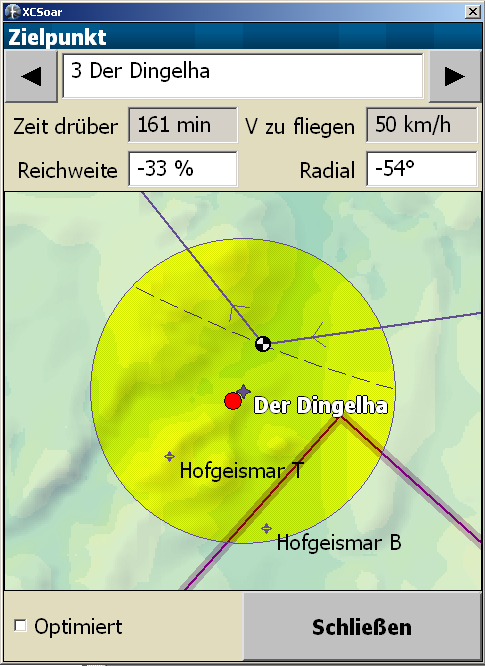
\includegraphics[angle=0,width=0.75\linewidth,keepaspectratio='true']{figures/aat-target.png}
%}
\end{center}
\achtung \item  Wenn nach dem Start unter \menulabel{\bmenut{Nav}{1/2}\blink\bmenut{Wende}{bereit}} angeklickt wurde, schaltet \xc bei Einflug in den Sektor
automatisch zum nächsten Wendepunkt um.
Sollte dieser Punkt nicht ideal sein, so kann hier mit \bmenut{Wende}{verschieben}  die Automatik ausgeschaltet werden und anschließend
manuell mit anschließend mit \bmenut{Nächster}{Wendepunkt} angeflogen und navigiert werden. Auch diese Speil kann beliebeig oft wiederholt werden, bis die optimalen Punkte erreicht sind.
Die dabei berechneten Werte werden unverzüglich in den entsprechenden InfoBoxen dargestellt.
\item Wenn ''AutoZoom'' aktiviert ist, wird die Karte automatisch rein- und rauszoomen, sobald Du Dich der Area und
dem entsprechenden Wendepunkt näherst.
\item  Einstellung und Nachjustierung  des MC-Wertes oder aber Einstellen von  \button{MacCready-Auto}.
Wenn der MC-Mode auf ''Endanflug'' oder aber ''Beides'' eingestellt wurde, wird der Rechner die optimale Sollfahrt vorgeben und den MC-Wert auf
den minimal benötigten Steigwert  stellen, um nach Hause zu kommen.
Dies unter Berücksichtigung der ''AAT-Differenzzeit'' um ja nicht zu früh zu Hause anzukommen.
\item  Anpassen von Mücken und Ballast
\item  Wenn benötigt, Anpassungen im \button{Analyse} Dialog vornehmen.
\item  Wenn benötigt, im \button{Status}-Dialog nachschauen, um Info bzgl.  Startzeit,
bislang abgelaufenen Zeit der Aufgabe, mittlerer Überlandgeschwindigkeit etc.\ zu kontrollieren.
\end{enumerate}

\subsection*{Nach der Landung landing}
Wie bereits  beschrieben in Kap.~\ref{sec:local-flight}.
